\documentclass[../../main]{subfiles}

\input{section_header.tex}

\begin{document}

\section{Data Processing Systems} \label{sec:}

All around us we are surrounded by different systems that constantly
engaged in different activities. These systems range from a home thermostat
to an industry grade quality testing machine. But they all have
one thing in common. They all take in some form of data, they process this
data, and take some kind of action based on the extracted information.

%% insert an flow chart showing the same

\begin{figure}
    \centering
    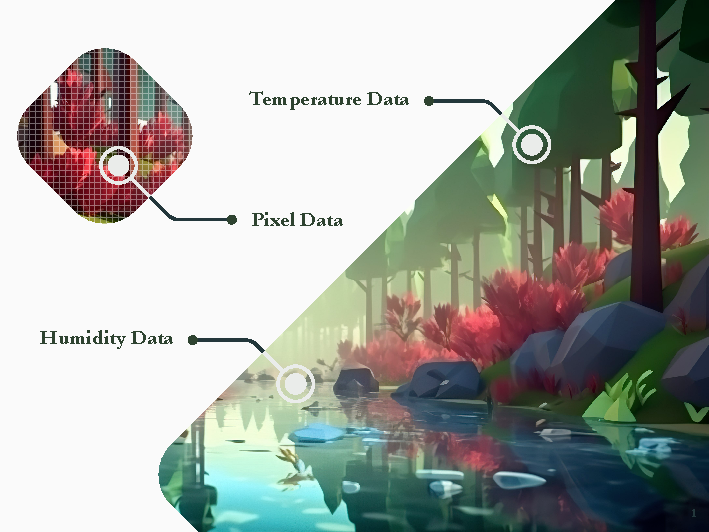
\includegraphics [
        max width = \IGXMaxWidth,
        max height = 0.3\textheight,
        \IGXDefaultOptionalArgs,
    ] {pics/different_kinds_of_data.pdf}
    \captionof{figure} {Different types of data surrounding us.}
    \label{fig:differentKindsOfData}
\end{figure}

As we can see from figure \ref{fig:differentKindsOfData}, there are different
kinds of data. Some are easily comprehensible and others that are a bit hard to
comprehend. Image data are such complex data forms. In order to properly make
use of the data, we need to somehow extract the useful information out them.

%% insert an flow chart showing the same

\end{document}
